\documentclass[usenames,dvipsnames,tikz]{standalone}
%\usepackage{xcolor}
\colorlet{tBlue}{RoyalBlue!35!Cerulean}
\colorlet{tRed}{Red}
%\usepackage{tikz}
%\usepackage{standalone}
\begin{document}
	
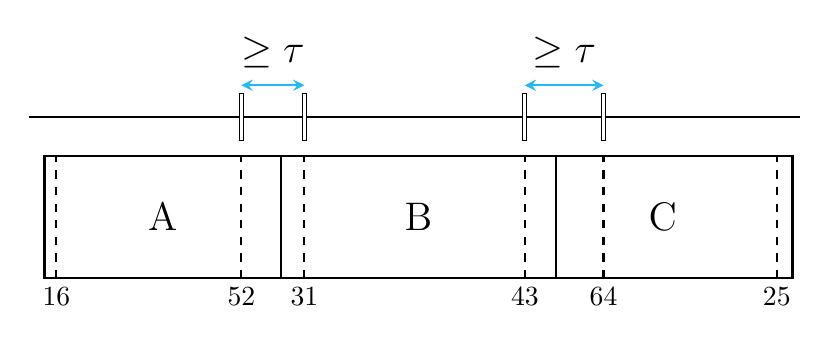
\begin{tikzpicture}
%\draw [help lines] (-1,-2) grid (17,5);

%-----------------
%red line first so that they appear under black lines


%3 items ordered
\draw [thick] (0,0) rectangle (9.5,1.55);
%between items A and B
\draw [thick] (3,0) -- (3,1.55);
%between items B and C
\draw [thick] (6.5, 0) -- (6.5,1.55);

%labels for items A, B and C
\node at (1.5,0.775) {\Large{A}};
\node at (4.75,0.775) {\Large{B}};
\node at (7.85,0.775) {\Large{C}};

%score lines and score width labels for item A
\draw [thick, dashed] (0.15,0) -- (0.15,1.55); %1
\draw [thick, dashed] (2.5,0) -- (2.5,1.55); %5
%\node [below] at (7.075,0) {1};
%\node [below] at (9.75,0) {5};
\node [below] at (0.15,0) {$16$};
\node [below] at (2.5,0) {$52$};

%score lines and score width labels for item B
\draw [thick, dashed] (3.3,0) -- (3.3,1.55); %3
%\draw [thick, red, dashed] (13.1,0) -- (12.1,1.55); %4 moved to top
%\node [below] at (10.15,0) {3};
\draw [thick, dashed] (6.1,0) -- (6.1,1.55); %43
\node [below] at (3.3,0) {$31$};
\node [below] at (6.1,0) {$43$};

%score lines and score width labels for item C
%\draw [thick, red, dashed] (13.7,0) -- (12.7,1.55); %2 moved to top
\draw [thick, dashed] (7.1,0) -- (7.1,1.55); %6
\draw [thick, dashed] (9.3,0) -- (9.3,1.55); %2
%\node [below] at (13.6,0) {\textcolor{tRed}{2}};
%\node [below] at (16.2,0) {6};
\node [below] at (7.1,0) {$64$};
\node [below] at (9.3,0) {$25$};

%------------------

%Bar with knives 
\draw [thick] (-0.2,2.05) -- (9.6,2.05);

%knives for items A and B
\filldraw[fill=white, draw=black, thin] (2.475,1.75) rectangle (2.525,2.35);
\filldraw[fill=white, draw=black, thin] (3.275,1.75) rectangle (3.325,2.35);
%\draw [thick] (9.5,1.75) -- (9.5,2.35);
%\draw [thick] (10.3,1.75) -- (10.3,2.35);

%knives for items B and C
\filldraw[fill=white, draw=black, thin] (6.075,1.75) rectangle (6.125,2.35);
\filldraw[fill=white, draw=black, thin] (7.075,1.75) rectangle (7.125,2.35);
%\draw [thick] (13.1,1.75) -- (13.1,2.35);
%\draw [thick] (13.7,1.75) -- (13.7,2.35);


%constraint label for score widths between items A and B (feasible, >= tau)
\draw [thick, <->, >=stealth, tBlue] (2.5, 2.45) -- (3.3, 2.45);
\node [above] at (2.9,2.55) {\Large{$\geq \tau$}};

%constraint label for score widths between items B and C (infeasible, < tau)
\draw [thick, <->,>=stealth, tBlue] (6.1, 2.45) -- (7.1, 2.45);
\node [above] at (6.6,2.55) {\Large{$\geq \tau$}};

%\draw [<->] (3.5,2.2) -- (4.5,2.2);
%\node at (4, -.4) {\scriptsize $\geq \tau$};

\end{tikzpicture}
	
\end{document}